\documentclass[conference]{IEEEtran}
\usepackage[utf8]{inputenc}
\usepackage[T1]{fontenc}
\usepackage{graphicx}
\usepackage{amsmath}
\usepackage{url}
\usepackage{lmodern}
\renewcommand{\rmdefault}{lmr}
\renewcommand{\sfdefault}{lmss}
\renewcommand{\ttdefault}{lmtt}

\hyphenation{evasão acadêmica micro-dados}

\begin{document}

\title{Comparação Auditada de Modelos de Aprendizado de Máquina para Predição de Alto Risco de Evasão em Cursos do Ensino Superior Brasileiro}

\author{
\IEEEauthorblockN{João Pedro, Luiz Miguel, Victor Conde, Gabriel Veloso, and Gabriel Albertan}
\IEEEauthorblockA{Centro de Informática --- Universidade Federal de Pernambuco (CIn-UFPE)}
}

\maketitle

\begin{abstract}
A evasão acadêmica constitui fenômeno multifatorial com impacto institucional, econômico e social. Este trabalho investiga a capacidade preditiva de cinco classificadores---Regressão Logística, Árvore de Decisão, Máquina de Vetores de Suporte (SVM), Rede Neural (MLP) e Naive Bayes (ComplementNB)---sobre microdados do Censo da Educação Superior 2024 (INEP), com alvo binário \texttt{ALTO\_RISCO\_EVASAO} (taxa de evasão $\geq 20\%$). Após auditoria metodológica que corrigiu a seleção de limiar de decisão (índice de Youden restrito ao intervalo $[0{,}2; 0{,}8]$), incorporou verificações de sanidade por fold e comparou os modelos a baselines triviais, constatou-se que conclusões prévias que favoreciam a Regressão Logística (Recall $\approx 0{,}999$) decorriam de limiares degenerados, e não de superioridade discriminativa. Sob protocolo validado (amostra estratificada de 30.000 cursos, validação cruzada 5-fold), a Árvore de Decisão obteve o melhor equilíbrio global (Accuracy $= 0{,}800$, Recall $= 0{,}768$, ROC-AUC $= 0{,}869$), seguida de desempenho estatisticamente equivalente do SVM (teste de Wilcoxon pareado em Recall: $p = 0{,}625$). A Rede Neural apresentou ROC-AUC competitivo ($0{,}869$) e maior PR-AUC ($0{,}883$), enquanto o Naive Bayes falhou em sensibilidade (Recall $= 0{,}047$) no pipeline unificado. Os resultados evidenciam que métricas dependentes de limiar devem ser interpretadas em conjunto com ROC-AUC, matriz de confusão e baselines, sob pena de conclusões metodologicamente inválidas.
\end{abstract}

\begin{IEEEkeywords}
Evasão acadêmica, aprendizado de máquina, INEP, classificação binária, auditoria metodológica, árvores de decisão.
\end{IEEEkeywords}

%==============================================================================
\section{Introdução}
%==============================================================================

\subsection{Contexto}
A evasão acadêmica designa a interrupção prematura da trajetória formativa do estudante antes da conclusão do curso, seja por desligamento, abandono ou trancamento prolongado. No contexto do ensino superior brasileiro, o fenômeno compromete a eficiência institucional, reduz a taxa de formação de capital humano qualificado e impacta indicadores de avaliação de políticas públicas, incluindo o Sistema Nacional de Avaliação da Educação Superior (Sinaes) e os instrumentos de regulação conduzidos pelo Instituto Nacional de Estudos e Pesquisas Educacionais Anísio Teixeira (INEP).

Do ponto de vista econômico, a evasão implica subutilização de vagas, custos irrecuperáveis de infraestrutura e perda de retorno sobre investimentos públicos e privados em educação. Socialmente, a não conclusão do curso pode restringir mobilidade ocupacional, perpetuar desigualdades e afetar a autopercepção de sucesso educacional dos estudantes. Por essas razões, a evasão deixou de ser tratada apenas como problema pedagógico individual e passou a ser compreendida como desafio estratégico de gestão institucional, demandando instrumentos de monitoramento, alerta precoce e alocação de recursos de permanência.

\subsection{Motivação}
A predição de risco de evasão em nível agregado (curso ou cohort) permite que gestores identifiquem contextos vulneráveis antes que o processo de abandono se consolide. Modelos preditivos baseados em dados censitários podem apoiar a priorização de programas de apoio psicopedagógico, revisão de políticas de ingresso, ajustes de oferta (turno, modalidade, financiamento) e avaliação de impacto de intervenções. Contudo, a utilidade prática desses modelos depende não apenas da acurácia global, mas da capacidade de detectar verdadeiros casos de alto risco (Recall) sem gerar alarmes espúrios em massa (controle de falsos positivos e de degenerescência do limiar).

\subsection{Dados educacionais e mineração de dados}
Os microdados do Censo da Educação Superior disponibilizados pelo INEP constituem fonte pública de elevado valor analítico, por reunirem informações demográficas, estruturais e de fluxo acadêmico em escala nacional. A mineração de dados educacionais (Educational Data Mining --- EDM) e a aprendizagem analítica em larga escala (Learning Analytics) têm explorado tais bases para modelagem de desempenho, evasão e permanência \cite{romero2020}. A aplicação de aprendizado de máquina a políticas educacionais exige, entretanto, rigor metodológico na definição do alvo, no pré-processamento sem vazamento de informação e na avaliação com métricas adequadas ao custo assimétrico dos erros.

\subsection{Objetivos e hipótese}
\textbf{Objetivo geral:} comparar, sob protocolo auditado e reprodutível, o desempenho de cinco famílias de classificadores na identificação de cursos com alto risco de evasão a partir dos microdados INEP 2024.

\textbf{Objetivos específicos:}
\begin{enumerate}
    \item implementar pipeline unificado de pré-processamento e validação cruzada estratificada;
    \item auditar a seleção de limiar de decisão e detectar métricas artificialmente infladas;
    \item ranquear modelos com base em métricas validadas e baselines triviais;
    \item analisar interpretabilidade e aplicabilidade da Árvore de Decisão como estudo de caso.
\end{enumerate}

\textbf{Hipótese implícita:} modelos com maior capacidade discriminativa (ROC-AUC) e Recall sustentado por especificidade não degenerada superarão baselines triviais e serão preferíveis a classificadores cuja aparente superioridade dependa exclusivamente de limiares extremos.

%==============================================================================
\section{Fundamentação Teórica}
%==============================================================================

\subsection{Regressão Logística}
A Regressão Logística modela a probabilidade de pertencimento à classe positiva mediante função logística sobre combinação linear das features \cite{hosmer2013}. É interpretável via odds ratios e computacionalmente eficiente. Suas limitações incluem a hipótese de separabilidade aproximadamente linear no espaço de atributos e sensibilidade a multicolinearidade e outliers. Em problemas com fronteiras não lineares e interações entre variáveis socioeconômicas, sua capacidade expressiva pode ser insuficiente, o que deve refletir-se em ROC-AUC moderado, independentemente do Recall observado em um limiar específico.

\subsection{Árvores de Decisão}
Árvores de decisão realizam particionamento recursivo do espaço de atributos, maximizando ganho de informação (entropia ou índice de Gini) em cada nó \cite{breiman1984}. Oferecem interpretabilidade direta por regras SE-ENTÃO e toleram features heterogêneas após codificação. O principal risco é o \textit{overfitting}, mitigado por poda (\textit{ccp\_alpha}), restrições de profundidade e tamanho mínimo de folha. Em contextos de política educacional, a transparência das regras é vantagem operacional relevante.

\subsection{Máquinas de Vetores de Suporte (SVM)}
A SVM busca o hiperplano de separação que maximiza a margem entre classes, podendo empregar kernels (e.g., RBF) para fronteiras não lineares \cite{cortes1995}. São reconhecidas pela robustez em espaços de alta dimensão e boa generalização quando hiperparâmetros são adequadamente calibrados. A interpretabilidade é inferior à das árvores, e o custo computacional cresce com o tamanho da amostra, embora ainda viável na escala deste estudo.

\subsection{Redes Neurais}
Perceptrons multicamadas (MLP) aproximam funções não lineares por composição de transformações afins e ativações \cite{haykin2009}. Possuem capacidade expressiva elevada, porém demandam tuning de arquitetura, regularização e inicialização. Em dados tabulares com amostra moderada, podem igualar ou superar modelos clássicos em métricas de ranking (ROC-AUC), com custo de opacidade decisória.

\subsection{Naive Bayes}
Classificadores Naive Bayes assumem independência condicional entre features dado a classe, estimando likelihoods com suavização de Laplace \cite{domingos2012}. O ComplementNB foi projetado para classes desbalanceadas e representações esparsas. Em dados tabulares com forte correlação entre atributos derivados de contagens INEP, a violação da independência pode comprometer a estimativa posterior, especialmente na classe positiva.

\subsection{Métricas de avaliação}
Seja $TP$, $FP$, $FN$, $TN$ os elementos da matriz de confusão. Accuracy mede a fração de acertos globais, mas é insuficiente em cenários balanceados artificialmente ou quando classes têm custos assimétricos. Precision ($TP/(TP+FP)$) quantifica a confiabilidade dos alertas; Recall ($TP/(TP+FN)$) quantifica a cobertura dos casos positivos. O F1-score harmoniza Precision e Recall, mas permanece dependente do limiar de decisão. A ROC-AUC resume a capacidade de discriminação ao variar o limiar, enquanto a PR-AUC é informativa em prevalências desafiadoras \cite{fawcett2006}. Neste estudo, a evasão é tratada como evento crítico a ser detectado; portanto, Recall e ROC-AUC possuem peso analítico superior à Accuracy isolada.

%==============================================================================
\section{Metodologia}
%==============================================================================

\subsection{Dataset e definição do alvo}
Utilizaram-se microdados de cadastro de cursos do Censo da Educação Superior 2024 (\texttt{MICRODADOS\_CADASTRO\_CURSOS\_2024.CSV}), com separador ponto-e-vírgula e codificação Latin-1. A variável resposta \texttt{ALTO\_RISCO\_EVASAO} foi definida como indicador binário de taxa de evasão $\geq 20\%$, calculada a partir de desligamentos e trancamentos sobre ingressantes ($QT\_ING > 0$). Foram derivadas nove variáveis de proporção (e.g., taxa de conclusão, proporção EAD, índices de financiamento) e selecionadas oito atributos categóricos institucionais codificados por \textit{Label Encoding}.

\subsection{Amostragem}
Extraiu-se amostra estratificada de $N = 30\,000$ cursos ($15\,000$ por classe), fixando prevalência em $50\%$ para evitar que métricas fossem dominadas por desbalanceamento extremo e para tornar explícita a comparação com baselines triviais (Accuracy $= 0{,}5$, Recall $= 1{,}0$ para classificador ``sempre positivo''). A amostragem estratificada preserva representatividade de ambas as classes e estabiliza a variância das métricas entre folds \cite{kohavi1995}, ao custo de não refletir a distribuição natural populacional---limitação explicitada na Seção~\ref{sec:ameacas}.

\subsection{Pré-processamento}
O pipeline por fold compreende: (i) imputação de ausentes pela moda, ajustada no treino; (ii) codificação ordinal de categorias no treino com mapeamento de categorias não vistas para valor reservado; (iii) seleção de features com $|\rho| \geq 0{,}05$ em relação ao alvo; (iv) padronização (\texttt{StandardScaler}), exceto ComplementNB (\texttt{MinMaxScaler}). O ajuste exclusivo no treino de cada fold previne vazamento de informação. A seleção por correlação reduz dimensionalidade e ruído, mas pode omitir variáveis preditivas não lineares; trata-se de compromisso interpretável entre parcimônia e completude.

\subsection{Modelos e hiperparâmetros}
Hiperparâmetros fixos provenientes dos experimentos originais e consolidados em \texttt{analysis/audit/evaluator.py}: Regressão Logística ($L_1$, $C=10$), Árvore de Decisão (entropia, \textit{max\_depth}=15, \textit{ccp\_alpha}$\approx 0{,}00435$, \textit{class\_weight} assimétrico), SVM (RBF, $C \approx 3{,}15$, $\gamma \approx 5{,}67$), MLP (64 neurônios, ReLU, SGD) e ComplementNB ($\alpha \approx 0{,}161$, \textit{norm}=True com SMOTE apenas no treino). Não houve reexecução de \textit{grid search} na validação final.

\subsection{Validação cruzada e calibração de limiar}
Adotou-se Stratified K-Fold com $K=5$ e \textit{shuffle} ($seed=42$). Em cada fold, $20\%$ do treino foi reservado para calibração do limiar, evitando que o conjunto de teste influenciasse a escolha do ponto de corte---prática alinhada à literatura de avaliação honesta \cite{kohavi1995}.

\subsubsection{Problema dos limiares degenerados}
A função original \texttt{encontrar\_melhor\_threshold} maximizava F1 no intervalo $[0{,}01; 0{,}99]$. Em classificadores com scores mal calibrados ou com massa probabilística concentrada em valores baixos, o ótimo de F1 frequentemente ocorre em limiares $\rightarrow 0$, classificando quase todas as instâncias como positivas. Nesse regime, Recall $\rightarrow 1$, mas $TN \rightarrow 0$ e Accuracy $\rightarrow$ prevalência da classe positiva. Para amostra balanceada ($50\%$), obtém-se Accuracy $\approx 0{,}5$ com aparente ``excelência'' em Recall---indistinguível do baseline trivial ``sempre positivo''. Esse fenômeno explica o Recall 0{,}999 da Regressão Logística pré-auditoria: não refletia poder discriminativo, mas colapso do limiar.

\subsubsection{Critério de Youden restrito}
A auditoria substituiu a maximização cega de F1 pelo índice de Youden $J = \text{sensibilidade} + \text{especificidade} - 1$, que busca explicitamente equilíbrio entre $TP$ e $TN$. O intervalo $[0{,}2; 0{,}8]$ foi adotado porque: (i) limiares $< 0{,}2$ continuavam a produzir taxas de positivos previstos incompatíveis com prevalência calibrada; (ii) limiares $> 0{,}8$ geravam Recall insuficiente para o problema de detecção de risco; (iii) o intervalo central força soluções operacionalmente plausíveis. Critérios adicionais rejeitam limiares cuja taxa de positivos previstos exceda $1{,}5\times$ a prevalência no conjunto de calibração, com \textit{fallback} em $0{,}5$ quando nenhum limiar satisfaz as restrições.

\subsection{Protocolo de sanidade}
Por fold, executaram-se seis verificações: (1) consistência da matriz de confusão; (2) comparação com classificadores triviais; (3) plausibilidade do limiar; (4) detecção do padrão Accuracy $\approx$ Precision com Recall elevado; (5) coerência entre ROC-AUC/PR-AUC e métricas no limiar; (6) sustentação para conclusões de excelência. Baselines ``Sempre Positivo'' e ``Sempre Majoritário'' foram incluídos no ranking (Score composto $= 0{,}775$).

%==============================================================================
\section{Resultados}
%==============================================================================

A Tabela~\ref{tab:metrics} consolida métricas validadas (média de cinco folds, recalculadas a partir de \texttt{validated\_metrics.csv} com consistência entre matriz de confusão e métricas reportadas, $\Delta < 0{,}002$).

\begin{table}[!t]
\centering
\caption{Métricas validadas sob protocolo auditado}
\label{tab:metrics}
\begin{tabular}{lccccc}
\hline
\textbf{Modelo} & \textbf{Acc.} & \textbf{Prec.} & \textbf{Rec.} & \textbf{F1} & \textbf{AUC} \\
\hline
Árvore de Decisão & 0.800 & 0.824 & 0.768 & 0.793 & 0.869 \\
SVM & 0.796 & 0.811 & 0.773 & 0.791 & 0.822 \\
Rede Neural & 0.800 & 0.831 & 0.754 & 0.790 & 0.869 \\
Regressão Log. & 0.660 & 0.734 & 0.503 & 0.596 & 0.699 \\
Naive Bayes & 0.519 & 0.841 & 0.047 & 0.089 & 0.593 \\
\hline
Baseline trivial  & 0.500 & 0.500 & 1.000 & 0.667 & 0.500 \\
\hline
\end{tabular}
\end{table}

Com pesos iguais ($20\%$ para Accuracy, Precision, Recall, F1 e ROC-AUC), a Árvore de Decisão lidera (Score $= 0{,}811$), seguida da Rede Neural ($0{,}809$) e SVM ($0{,}799$). No ranking auditado com ênfase em Recall (peso $45\%$), Árvore e SVM permanecem no topo; Wilcoxon pareado em Recall entre ambos: $p = 0{,}625$ (sem significância a $\alpha = 0{,}05$).

\begin{figure}[!t]
\centering
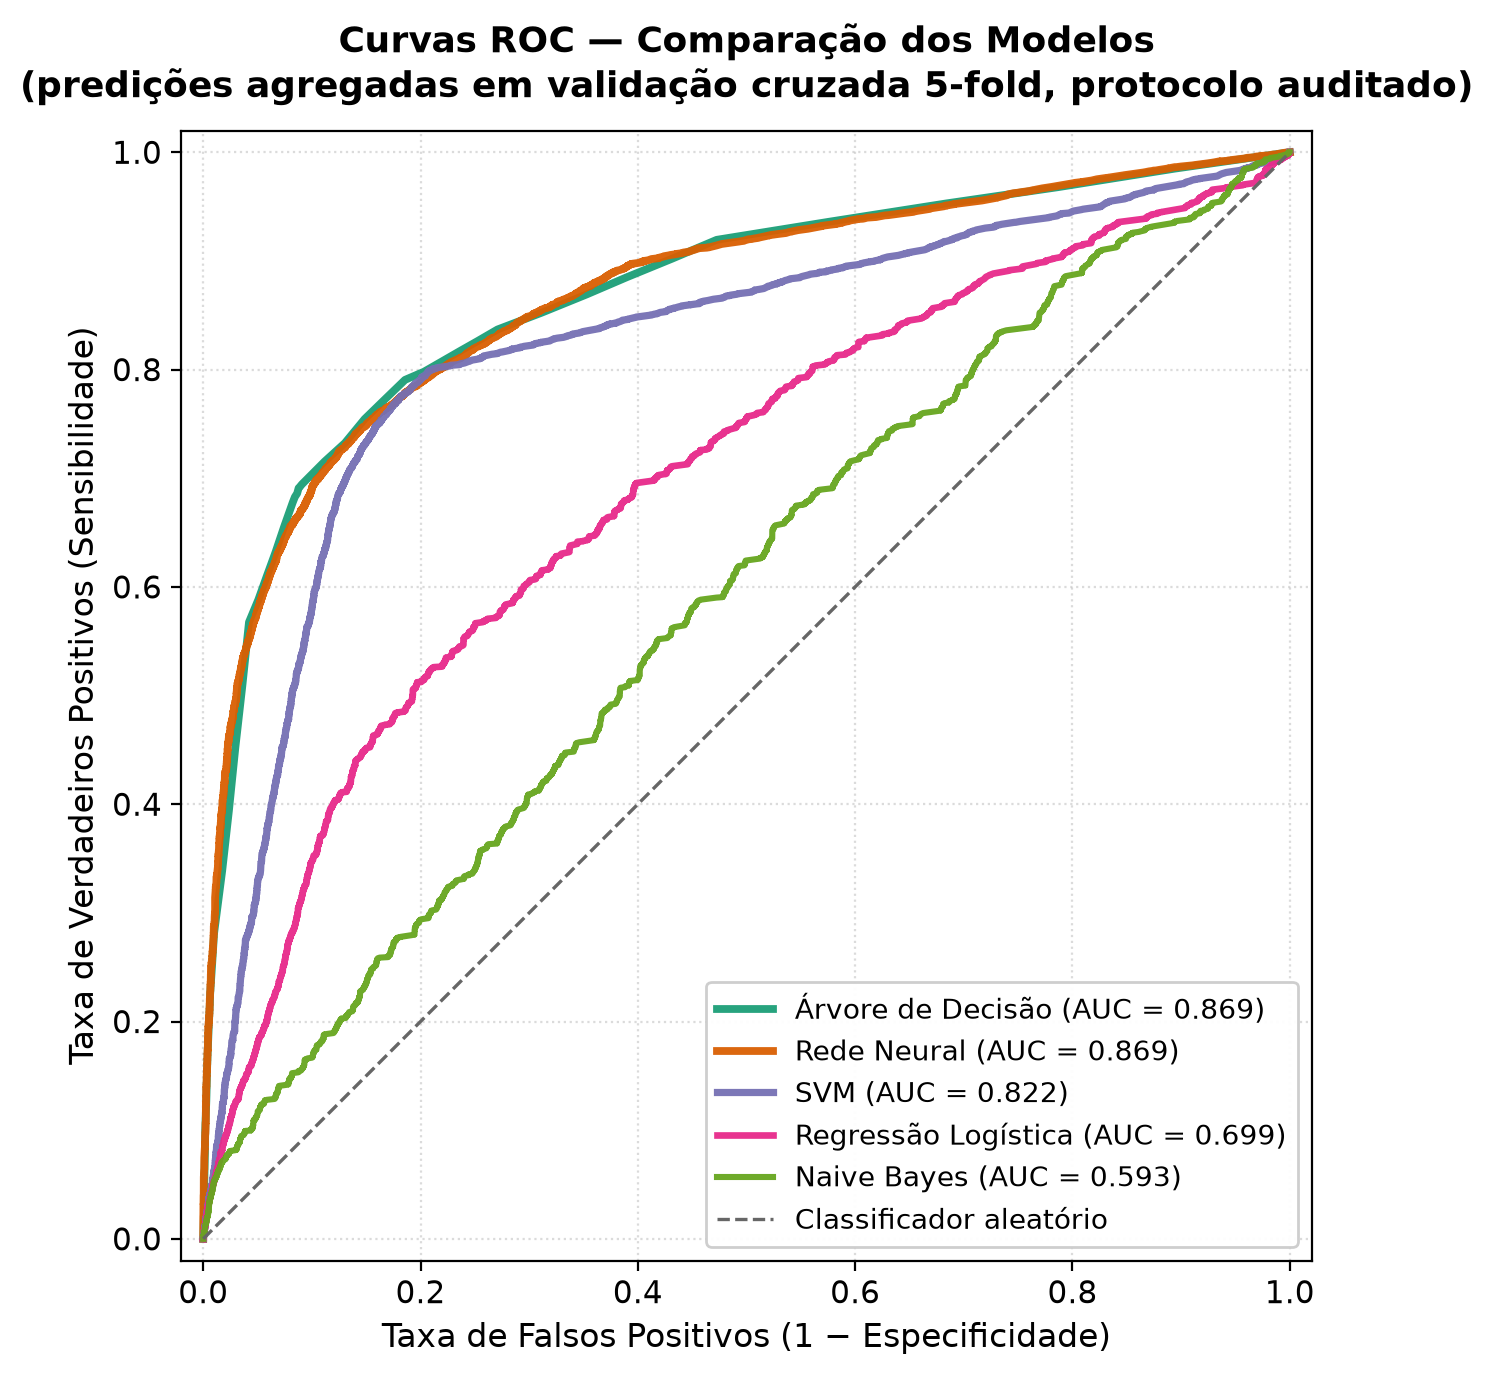
\includegraphics[width=\linewidth]{validation/roc_comparison.png}
\caption{Curvas ROC comparativas --- predições agregadas em validação cruzada 5-fold (protocolo auditado). AUC na legenda conforme \texttt{validated\_metrics.csv}.}
\label{fig:roc}
\end{figure}

A Figura~\ref{fig:roc} corrobora a separação hierárquica: Árvore e Rede Neural ($\text{AUC} \approx 0{,}869$) discriminam melhor que Regressão Logística ($0{,}699$) e Naive Bayes ($0{,}593$). O TN médio por fold (Árvore: 2497; SVM: 2457; Naive Bayes: 2973 com $TP$ médio 140) evidencia que alto TN isolado não implica bom modelo se acompanhado de FN massivo.

%==============================================================================
\section{Análise Comparativa dos Modelos}
%==============================================================================

A análise comparativa transcende o ranqueamento numérico: interpreta \textit{por que} cada família algorítmica produziu o padrão observado de erros, como a auditoria de limiar alterou a hierarquia de modelos e quais implicações práticas decorrem para a implantação em contexto de gestão educacional. As discussões a seguir referem-se exclusivamente às métricas validadas (Tabela~\ref{tab:metrics}), com médias sobre cinco folds e limiar calibrado por índice de Youden restrito. Cada subseção inclui a matriz de confusão agregada correspondente (Figuras~\ref{fig:cm_lr}--\ref{fig:cm_nb}), exportada de \texttt{results/validation/}.

\subsection{Regressão Logística}
No ranking pré-auditoria, a Regressão Logística aparecia como melhor modelo (Recall $= 0{,}999$, Score composto $= 0{,}896$). Após correção metodológica, seu Recall caiu para 0{,}503, F1 para 0{,}596 e ROC-AUC permaneceu em 0{,}699, posicionando o classificador abaixo dos três líderes e apenas marginalmente acima do Naive Bayes em capacidade discriminativa global.

\textbf{Por que inicialmente parecia superior?} A maximização cega de F1 em $[0{,}01; 0{,}99]$ favorecia limiares extremamente baixos ($\approx 0{,}01$), nos quais a função logística atribuía rótulo positivo a quase todos os cursos. Matematicamente, isso maximiza $TP$ e, portanto, Recall, mas aniquila $TN$: o classificador torna-se funcionalmente equivalente ao baseline ``sempre positivo'' (Recall $= 1{,}0$, Accuracy $= 0{,}5$). A coincidência entre Accuracy e Precision elevadas com Recall próximo de $1$ constitui, na auditoria, sinal de alerta (\textit{sanity check} 4), não evidência de excelência preditiva.

\textbf{Por que deixou de ser a melhor opção após validação?} Porque o ROC-AUC ($0{,}699$) indica separação moderada entre classes no espaço de scores; a vantagem aparente em Recall era artefato de calibração, não de ranking superior. Com limiar restrito, a Regressão Logística passa a errar aproximadamente metade dos casos positivos ($FN$ elevado em relação aos líderes), enquanto sua Precision ($0{,}734$) não compensa a perda de sensibilidade. O TN médio (2450) é comparável ao da Árvore (2497), mas o TP médio (1510 vs.\ 2305) revela que a sensibilidade recuperada pelos líderes provém de melhor discriminação estrutural, não de limiar permissivo.

Do ponto de vista teórico, a hipótese de linearidade logística é plausível para relações monotônicas entre indicadores INEP e risco, porém insuficiente para capturar interações (e.g., alto ingresso combinado com baixa taxa de conclusão). A Regressão Logística permanece útil para inferência sobre direção de efeitos e comunicação com audiências acostumadas a odds ratios, mas não como líder operacional em detecção de alto risco sob protocolo rigoroso. A Figura~\ref{fig:cm_lr} evidencia $FN$ elevado (1490) frente aos líderes, confirmando perda de sensibilidade após auditoria de limiar.

\begin{figure}[!t]
\centering
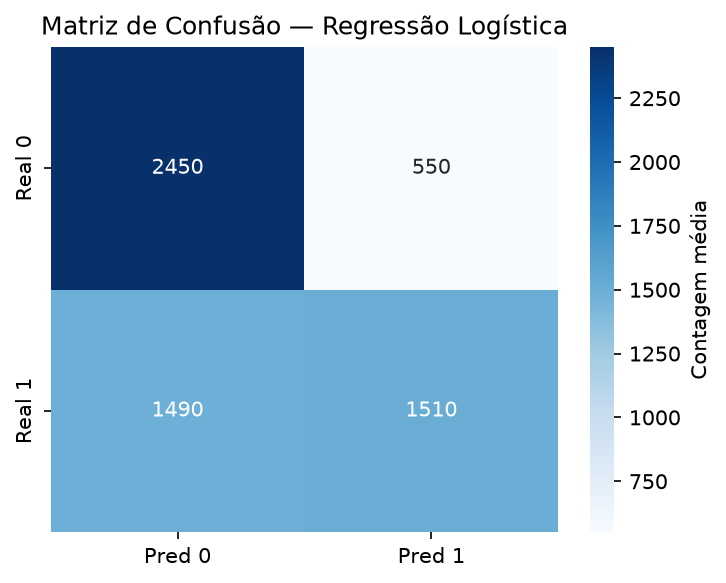
\includegraphics[width=\linewidth]{validation/confusion_matrix_regressao_logistica.png}
\caption{Matriz de confusão média (5 folds) --- Regressão Logística. Contagens médias por fold ($n_{teste}=6000$): $TN=2450$, $FP=550$, $FN=1490$, $TP=1510$.}
\label{fig:cm_lr}
\end{figure}

\subsection{Árvore de Decisão}
A Árvore de Decisão obteve o melhor equilíbrio entre Recall ($0{,}768$), Precision ($0{,}824$), F1 ($0{,}793$) e ROC-AUC ($0{,}869$), com TN médio 2497 e TP médio 2305 em conjunto de teste de $6000$ instâncias por fold. No ranking com pesos iguais ($20\%$ por métrica), lidera com Score 0{,}811; no ranking auditado com ênfase em Recall ($45\%$), mantém a primeira posição.

\textbf{Por que liderou o ranking?} Três fatores convergem. Primeiro, o particionamento recursivo modela interações e não linearidades sem engenharia manual de features, adequando-se a indicadores de fluxo (ingresso, matrícula, razões derivadas) que não se comportam linearmente em relação ao risco. Segundo, a poda via \textit{ccp\_alpha} e profundidade efetiva $5$ (Seção~\ref{sec:arvore}) limitam sobreajuste, preservando generalização entre folds (desvio padrão de Recall na ordem de centésimos). Terceiro, as probabilidades de folha, calibradas com limiar de Youden restrito, evitam a degenerescência observada na Regressão Logística: o modelo discrimina \textit{e} opera em ponto de corte equilibrado.

\textbf{Por que é solução prática?} Gestores educacionais podem inspecionar regras explícitas (\texttt{decision\_tree\_rules.txt}) e discutir políticas em termos de indicadores já monitorados pelo INEP---ingresso, matrícula, taxa de conclusão---sem depender de explicações pós-hoc. A implementação em \texttt{scikit-learn} \cite{pedregosa2011} é leve, treinamento rápido em $24\,000$ amostras por fold e inferência $O(\text{profundidade})$. O custo de interpretabilidade parcial (limiares em escala padronizada) é documentável e inferior ao de modelos de caixa-preta. A Figura~\ref{fig:cm_tree} ilustra equilíbrio entre $TP$ e $TN$ sem colapso de especificidade.

\begin{figure}[!t]
\centering
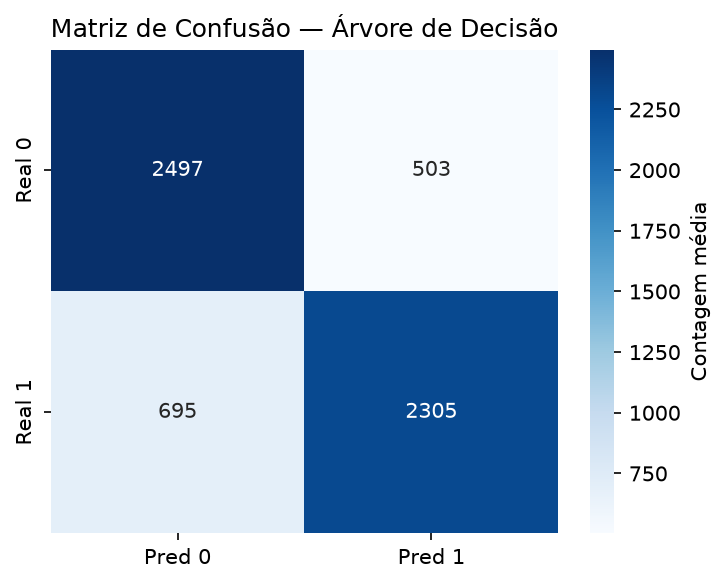
\includegraphics[width=\linewidth]{validation/confusion_matrix_arvore_de_decisao.png}
\caption{Matriz de confusão média (5 folds) --- Árvore de Decisão. Contagens médias por fold ($n_{teste}=6000$): $TN=2497$, $FP=503$, $FN=695$, $TP=2305$.}
\label{fig:cm_tree}
\end{figure}

\subsection{SVM}
A SVM apresentou métricas muito próximas à Árvore: Recall $0{,}773$ vs.\ $0{,}768$, Precision $0{,}811$ vs.\ $0{,}824$, F1 $0{,}791$ vs.\ $0{,}793$. O teste de Wilcoxon pareado em Recall entre ambos retornou $p = 0{,}625$, incompatível com rejeição da hipótese nula de igualdade de distribuições entre folds a $\alpha = 0{,}05$. Em termos práticos, as diferenças observadas podem decorrer de variância amostral, não de superioridade estrutural de um algoritmo sobre o outro.

O kernel RBF ($C \approx 3{,}15$, $\gamma \approx 5{,}67$) projeta os dados em espaço de dimensão elevada, permitindo fronteiras suaves que maximizam a margem entre classes. O ROC-AUC ($0{,}822$) é inferior ao da Árvore ($0{,}869$), sugerindo que, embora o desempenho no limiar calibrado seja equivalente, a ordenação global de scores da SVM é ligeiramente menos informativa---implicação relevante se a instituição priorizar triagem por score contínuo antes de fixar limiar operacional.

\textbf{Existe diferença prática entre SVM e Árvore?} Para detecção binária com limiar auditado, não de forma estatisticamente significativa. A distinção reside em governança: a Árvore oferece regras auditáveis; a SVM exige técnicas adicionais (e.g., LIME, SHAP) para explicação. Em ambientes com exigência regulatória de transparência, a Árvore é preferível; em pipelines automatizados de scoring com revisão humana posterior, a SVM é alternativa robusta e estável. A Figura~\ref{fig:cm_svm} confirma padrão de erros visualmente indistinguível do da Árvore.

\begin{figure}[!t]
\centering
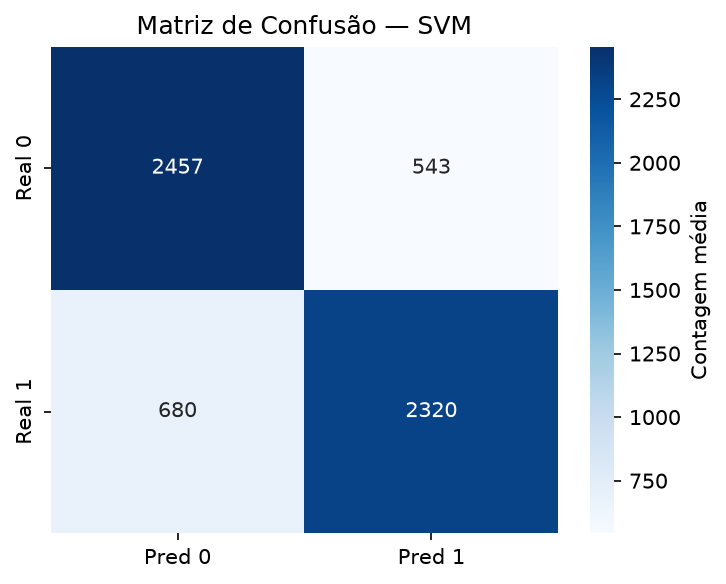
\includegraphics[width=\linewidth]{validation/confusion_matrix_svm.png}
\caption{Matriz de confusão média (5 folds) --- SVM. Contagens médias por fold ($n_{teste}=6000$): $TN=2457$, $FP=543$, $FN=680$, $TP=2320$.}
\label{fig:cm_svm}
\end{figure}

\subsection{Rede Neural}
O MLP (64 neurônios, ReLU, SGD) alcançou Accuracy $0{,}800$, Precision $0{,}831$ (a mais alta entre os cinco modelos), Recall $0{,}754$, F1 $0{,}790$, ROC-AUC $0{,}869$ e PR-AUC $0{,}883$ (máximo do conjunto). Posiciona-se em segundo lugar no ranking com pesos iguais (Score $0{,}809$), a $0{,}002 da Árvore---diferença desprezível no critério composto.

A rede combina capacidade expressiva não linear com regularização implícita do protocolo (validação cruzada, limiar restrito). O PR-AUC superior indica melhor compromisso precisão-revocação ao longo da curva de limiares, útil quando a prevalência operacional difere da amostra balanceada artificialmente. Contudo, o Recall no limiar único ($0{,}754$) fica abaixo da Árvore e da SVM: a rede é mais conservadora em positivos, privilegiando Precision.

\textbf{O ganho justifica a perda de interpretabilidade?} A resposta depende do caso de uso. Se o objetivo é ranking contínuo para priorização de visitas técnicas ou auditorias amostrais, o ganho em PR-AUC pode justificar o MLP como componente de \textit{ensemble} ou segundo opinador. Se o objetivo é formulação de políticas públicas com justificativa explícita perante conselhos e órgãos de controle, o ganho marginal ($< 2$ pontos percentuais em métricas principais) não compensa opacidade, custo de \textit{hyperparameter tuning} e risco de instabilidade ante re-treinamentos periódicos. Neste estudo, a Árvore permanece recomendada como modelo primário; a rede, como validação cruzada de robustez discriminativa. A Figura~\ref{fig:cm_rn} mostra $TN$ ligeiramente superior e $FN$ moderadamente maior que na Árvore, coerente com maior Precision e menor Recall.

\begin{figure}[!t]
\centering
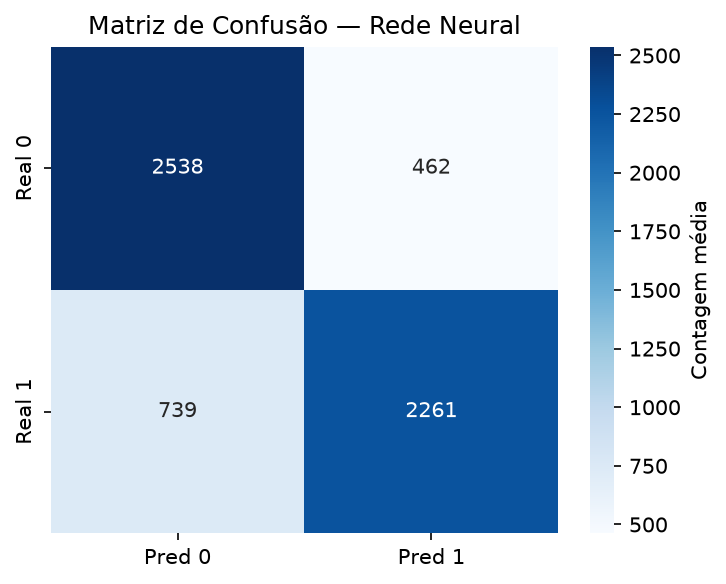
\includegraphics[width=\linewidth]{validation/confusion_matrix_rede_neural.png}
\caption{Matriz de confusão média (5 folds) --- Rede Neural. Contagens médias por fold ($n_{teste}=6000$): $TN=2538$, $FP=462$, $FN=739$, $TP=2261$.}
\label{fig:cm_rn}
\end{figure}

\subsection{Naive Bayes}
O ComplementNB exibiu o pior desempenho global: Accuracy $0{,}519$, Recall $0{,}047$, F1 $0{,}089$, ROC-AUC $0{,}593$. Paradoxalmente, apresentou a segunda maior Precision ($0{,}841$), apenas atrás da Rede Neural---padrão característico de classificador excessivamente conservador na classe positiva.

\textbf{Por que Recall extremamente baixo?} A hipótese de independência condicional é severamente violada: variáveis como \textit{QT\_ING}, \textit{QT\_MAT} e \textit{RAZAO\_ING\_MAT} são estruturalmente correlacionadas (ingresso determina parcialmente matrícula). O ComplementNB, projetado para representações esparsas de texto, estima likelihoods que, sob correlação forte, concentram massa probabilística na classe negativa. O resultado é TN médio elevado (2973) com TP médio crítico (140): o modelo quase nunca alerta alto risco, falhando em aproximadamente $95\%$ dos casos positivos.

O SMOTE aplicado apenas no treino do pipeline unificado não reestrutura as dependências entre features; apenas rebalanceia contagens de instâncias. A ROC-AUC ($0{,}593$) próxima de $0{,}5$ confirma discriminação fraca, independentemente de limiar. \textbf{Implicação prática:} o Naive Bayes, no protocolo atual, é inadequado para detecção de evasão; poderia, no máximo, servir como filtro de alta Precision em cascata (primeiro estágio conservador), mas isso exigiria redesenho arquitetural não avaliado neste trabalho. A Figura~\ref{fig:cm_nb} expõe o padrão crítico: $FN$ massivo (2860) com $FP$ mínimo (27), típico de classificador que quase nunca emite alerta de alto risco.

\begin{figure}[!t]
\centering
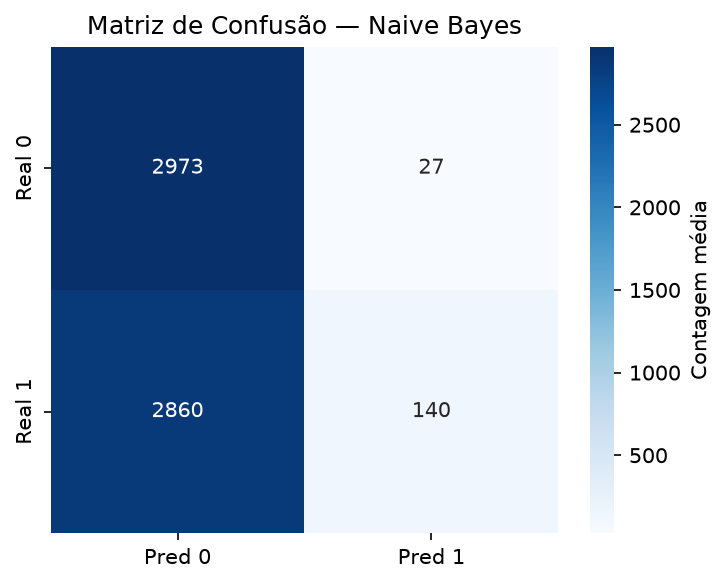
\includegraphics[width=\linewidth]{validation/confusion_matrix_naive_bayes.png}
\caption{Matriz de confusão média (5 folds) --- Naive Bayes. Contagens médias por fold ($n_{teste}=6000$): $TN=2973$, $FP=27$, $FN=2860$, $TP=140$.}
\label{fig:cm_nb}
\end{figure}

\subsection{Síntese comparativa}
A Tabela~\ref{tab:metrics}, a Figura~\ref{fig:roc} e as matrizes de confusão (Figuras~\ref{fig:cm_lr}--\ref{fig:cm_nb}) permitem hierarquizar os modelos em três faixas: (i) \textbf{tier operacional}---Árvore, SVM e Rede Neural, com ROC-AUC $\geq 0{,}82$ e Recall $\geq 0{,}75$; (ii) \textbf{tier intermediário}---Regressão Logística, com discriminação moderada e sensibilidade comprometida após auditoria; (iii) \textbf{tier inadequado}---Naive Bayes, com falha estrutural de sensibilidade. A auditoria de limiar foi determinante para revelar essa estrutura: sem ela, conclusões favoreceriam erroneamente a Regressão Logística. A escolha final entre os três primeiros deve privilegiar interpretabilidade (Árvore), equivalência estatística com menor AUC global (SVM) ou PR-AUC máximo (Rede Neural), conforme prioridades institucionais.

%==============================================================================
\section{Discussão}
%==============================================================================

\subsection{Sobre as métricas}
Accuracy isolada não conta toda a história: com prevalência $50\%$, um classificador trivial pode atingir $0{,}5$ sem valor preditivo. Neste problema, \textbf{Recall é operacionalmente central}, pois representa a fração de cursos de alto risco efetivamente sinalizados; contudo, Recall sem TN (especificidade) é enganoso---como demonstrado pela Regressão Logística pré-auditoria e pelo Naive Bayes pós-auditoria. O ROC-AUC complementa a análise ao medir qualidade global da ordenação por score, independentemente de um único limiar; discrepâncias entre Recall alto e AUC moderado sinalizam calibração inadequada.

\subsection{Sobre interpretabilidade}
Em educação, decisões algorítmicas afetam alocação de bolsas, monitoramento de cursos e imagem institucional. Gestores educacionais frequentemente necessitam justificar ações a conselhos e órgãos reguladores; modelos interpretáveis reduzem assimetria de informação entre equipe técnica e decisores. A Árvore de Decisão atende parcialmente a esse requisito, embora variáveis codificadas exijam documentação auxiliar.

\subsection{Sobre aplicabilidade}
Em cenário real com foco em detecção precoce e transparência, recomenda-se Árvore de Decisão ou SVM, priorizando a primeira quando a explicabilidade for mandatória. A Rede Neural é reserva para análises secundárias de ranking. Regressão Logística e Naive Bayes não devem liderar implantação sem reformulação metodológica substancial.

\subsection{Sobre robustez}
Os resultados são consistentes entre folds (variação pequena de Recall e F1), e a recalibração de métricas a partir da matriz de confusão confirmou coerência numérica. Não há evidência de instabilidade grave entre partições; a equivalência estatística Árvore--SVM sugere que a escolha final pode basear-se em critérios de governança (interpretabilidade, custo) mais que em ganho preditivo marginal.

%==============================================================================
\section{Estudo de Caso: Árvore de Decisão}
\label{sec:arvore}
%==============================================================================

\subsection{Estrutura e complexidade}
A árvore ajustada com hiperparâmetros auditados atingiu profundidade efetiva $5$ (limite configurado $15$), $19$ nós e $10$ folhas, com impureza média nas folhas $0{,}571$. A poda via \textit{ccp\_alpha} reduziu complexidade, mitigando sobreajuste enquanto preservou ROC-AUC elevado ($0{,}869$). A representação gráfica completa da árvore consta no Anexo (Figura~\ref{fig:tree}).

\subsection{Variáveis mais importantes}
A importância por Gini (top quatro) foi: \textit{RAZAO\_ING\_MAT} ($0{,}511$), \textit{QT\_ING} ($0{,}329$), \textit{QT\_MAT} ($0{,}114$), \textit{TAXA\_CONCLUSAO} ($0{,}046$). A razão ingresso/matrícula captura descompasso entre fluxo de entrada e base matriculada---possível indicador de instabilidade de cohort. Volume de ingressantes e matrículas reflete escala e dinâmica do curso; taxa de conclusão baixa pode sinalizar gargalos de permanência. Essas variáveis são plausíveis do ponto de vista teórico da evasão \cite{tinto2010}.

\subsection{Regras aprendidas e significado}
Exemplos de regras extraídas (\texttt{decision\_tree\_rules.txt}): quando \textit{QT\_ING} $\leq -0{,}12$ (ingresso abaixo da média padronizada) e \textit{RAZAO\_ING\_MAT} $\leq -1{,}05$, a folha prediz alto risco (\texttt{class: 1})---configuração compatível com descompasso entre entrada de alunos e base matriculada estável. Ramo alternativo: \textit{QT\_ING} $> -0{,}12$ com \textit{TAXA\_CONCLUSAO} $> -0{,}31$ também conduz a predição positiva, sugerindo que cursos com ingresso relativamente alto mas conclusão acima de um limiar ainda assim são sinalizados, possivelmente por interação com outras variáveis no caminho da árvore.

Quando \textit{RAZAO\_ING\_MAT} assume valores intermediários ($-1{,}05$ a $1{,}19$) e \textit{QT\_MAT} é baixo, predomina classe negativa (\texttt{class: 0}): cursos com matrícula reduzida e razão ingresso/matrícula moderada tendem a não ser classificados como alto risco. Os limiares estão em escala padronizada; a interpretação qualitativa requer referência às distribuições no treino. Ainda assim, as regras permitem diálogo entre analistas e gestores sobre quais indicadores INEP merecem monitoramento contínuo e em que combinações configuram alerta.

\subsection{Interpretabilidade e apoio à decisão}
Árvores são amplamente utilizadas em sistemas de apoio à decisão públicos por traduzirem políticas em critérios auditáveis. A limitação reside na instabilidade de árvores únicas pequenas ante perturbações dos dados; ensembles (Random Forest) poderiam aumentar robustez à custa de interpretabilidade global.

%==============================================================================
\section{Ameaças à Validade}
\label{sec:ameacas}
%==============================================================================

\subsection{Validade interna}
A amostragem balanceada $50/50$ facilita comparação e detecção de degenerescência, mas não representa prevalência populacional real de alto risco---métricas absolutas de Precision/Recall em produção podem diferir. O pré-processamento por fold minimiza vazamento; a seleção por correlação pode excluir preditores não lineares não correlacionados marginalmente. A calibração de limiar em subconjunto do treino introduz variância adicional, embora necessária para evitar otimismo no teste.

\subsection{Validade externa}
Os modelos foram estimados em snapshot de 2024; generalização para outros anos pressupõe estabilidade das relações estruturais e das definições INEP. Generalização para instituições específicas (micro em vez de agregado por curso) não foi avaliada. Resultados aplicam-se ao nível de agregação curricular do Censo.

\subsection{Limitações computacionais e metodológicas}
Não foram avaliados ensembles (Random Forest, XGBoost), validação temporal (\textit{train past, test future}) nem calibração probabilística pós-hoc (Platt, isotônica). O pipeline do Naive Bayes original (mediana, \textit{QT\_ING} $\geq 10$) difere do protocolo unificado, inviabilizando comparação histórica direta sem reexecução controlada.

%==============================================================================
\section{Conclusão}
%==============================================================================

Este estudo comparou cinco classificadores---Regressão Logística, Árvore de Decisão, SVM, Rede Neural (MLP) e Naive Bayes (ComplementNB)---para predição de alto risco de evasão em cursos do ensino superior brasileiro, a partir dos microdados do Censo INEP 2024. O alvo binário \texttt{ALTO\_RISCO\_EVASAO} (taxa de evasão $\geq 20\%$) foi modelado sob amostra estratificada de $30\,000$ cursos, validação cruzada 5-fold e protocolo de auditoria que corrigiu degenerescência na seleção de limiar de decisão.

\textbf{Síntese dos resultados.} A Árvore de Decisão obteve o melhor equilíbrio global (Accuracy $0{,}800$, Recall $0{,}768$, ROC-AUC $0{,}869$, Score composto $0{,}811$), seguida de desempenho estatisticamente equivalente da SVM em Recall (Wilcoxon: $p = 0{,}625$) e da Rede Neural em ROC-AUC e PR-AUC ($0{,}883$). A Regressão Logística, anteriormente classificada como melhor modelo do projeto (Recall $0{,}999$), foi rebaixada após auditoria para Recall $0{,}503$ e ROC-AUC $0{,}699$, evidenciando que a aparente superioridade decorria de limiares degenerados, não de melhor discriminação. O Naive Bayes falhou em sensibilidade (Recall $0{,}047$), inadequado para detecção operacional de alto risco.

\textbf{Justificativa da escolha final.} Recomenda-se a Árvore de Decisão como modelo primário quando interpretabilidade, desempenho equilibrado e conformidade com indicadores INEP são prioritários. A SVM constitui substituto válido em cenários de menor exigência explicativa. A Rede Neural pode complementar análises de ranking por PR-AUC, mas não justifica, neste dataset, a complexidade adicional como solução única.

\textbf{Contribuições.} (1) Comparação reprodutível de cinco famílias de modelos sob pipeline unificado; (2) demonstração empírica de que métricas dependentes de limiar (Recall, F1) podem induzir conclusões inválidas sem análise de TN, ROC-AUC e baselines triviais; (3) protocolo de auditoria replicável (Youden em $[0{,}2; 0{,}8]$, \textit{sanity checks}, recálculo de métricas a partir da matriz de confusão); (4) estudo de caso interpretativo da árvore, com variáveis de fluxo (\textit{RAZAO\_ING\_MAT}, \textit{QT\_ING}, \textit{TAXA\_CONCLUSAO}) alinhadas à literatura de permanência \cite{tinto2010}.

\textbf{Limitações.} Amostra parcial balanceada artificialmente ($50/50$); agregação por curso (não por estudante); snapshot temporal único (2024); ausência de ensembles e validação temporal; pipeline do Naive Bayes original difere do unificado.

\textbf{Trabalhos futuros.} Incorporar validação prospectiva (\textit{train past, test future}), calibração probabilística pós-hoc, explicações globais (SHAP), comparação com Random Forest e XGBoost sob o mesmo protocolo auditado, e avaliação de custo assimétrico de erros com participação de gestores institucionais.

%==============================================================================
\section*{Agradecimentos}
%==============================================================================

Os autores agradecem ao INEP pela disponibilização dos microdados do Censo da Educação Superior e ao CIn-UFPE pelo suporte acadêmico.


\begin{thebibliography}{99}

\bibitem{breiman1984}
L. Breiman, J. Friedman, R. Olshen, and C. Stone,
\emph{Classification and Regression Trees}.
Belmont, CA, USA: Wadsworth, 1984.

\bibitem{cortes1995}
C. Cortes and V. Vapnik,
``Support-vector networks,''
\emph{Machine Learning}, vol. 20, no. 3, pp. 273--297, 1995.

\bibitem{domingos2012}
P. Domingos and G. Hulten,
``Mining high-speed data streams,''
in \emph{Proc. ACM SIGKDD}, 2000, pp. 71--80.

\bibitem{fawcett2006}
T. Fawcett,
``An introduction to ROC analysis,''
\emph{Pattern Recognition Letters}, vol. 27, no. 8, pp. 861--874, 2006.

\bibitem{haykin2009}
S. Haykin,
\emph{Neural Networks and Learning Machines}, 3rd ed.
Upper Saddle River, NJ, USA: Prentice Hall, 2009.

\bibitem{hosmer2013}
D. W. Hosmer, S. Lemeshow, and R. X. Sturdivant,
\emph{Applied Logistic Regression}, 3rd ed.
Hoboken, NJ, USA: Wiley, 2013.

\bibitem{inep2024}
INEP,
\emph{Microdados do Censo da Educação Superior 2024}.
Brasília, DF, Brasil, 2024. [Online]. Available: \url{https://www.gov.br/inep}

\bibitem{kohavi1995}
R. Kohavi,
``A study of cross-validation and bootstrap for accuracy estimation and model selection,''
in \emph{Proc. IJCAI}, 1995, pp. 1137--1145.

\bibitem{pedregosa2011}
F. Pedregosa \emph{et al.},
``Scikit-learn: Machine learning in Python,''
\emph{Journal of Machine Learning Research}, vol. 12, pp. 2825--2830, 2011.

\bibitem{romero2020}
C. Romero and S. Ventura,
``Educational data mining and learning analytics: An updated survey,''
\emph{Wiley Interdisciplinary Reviews: Data Mining and Knowledge Discovery}, vol. 10, no. 3, e1355, 2020.

\bibitem{tinto2010}
V. Tinto,
\emph{Leaving College: Rethinking the Causes and Cures of Student Attrition}, 2nd ed.
Chicago, IL, USA: Univ. Chicago Press, 2010.

\end{thebibliography}

\clearpage
\onecolumn
\section*{Anexo: Árvore de Decisão}
\label{sec:arvore}
\vspace*{0.5em}
\begin{figure}[!t]
\centering
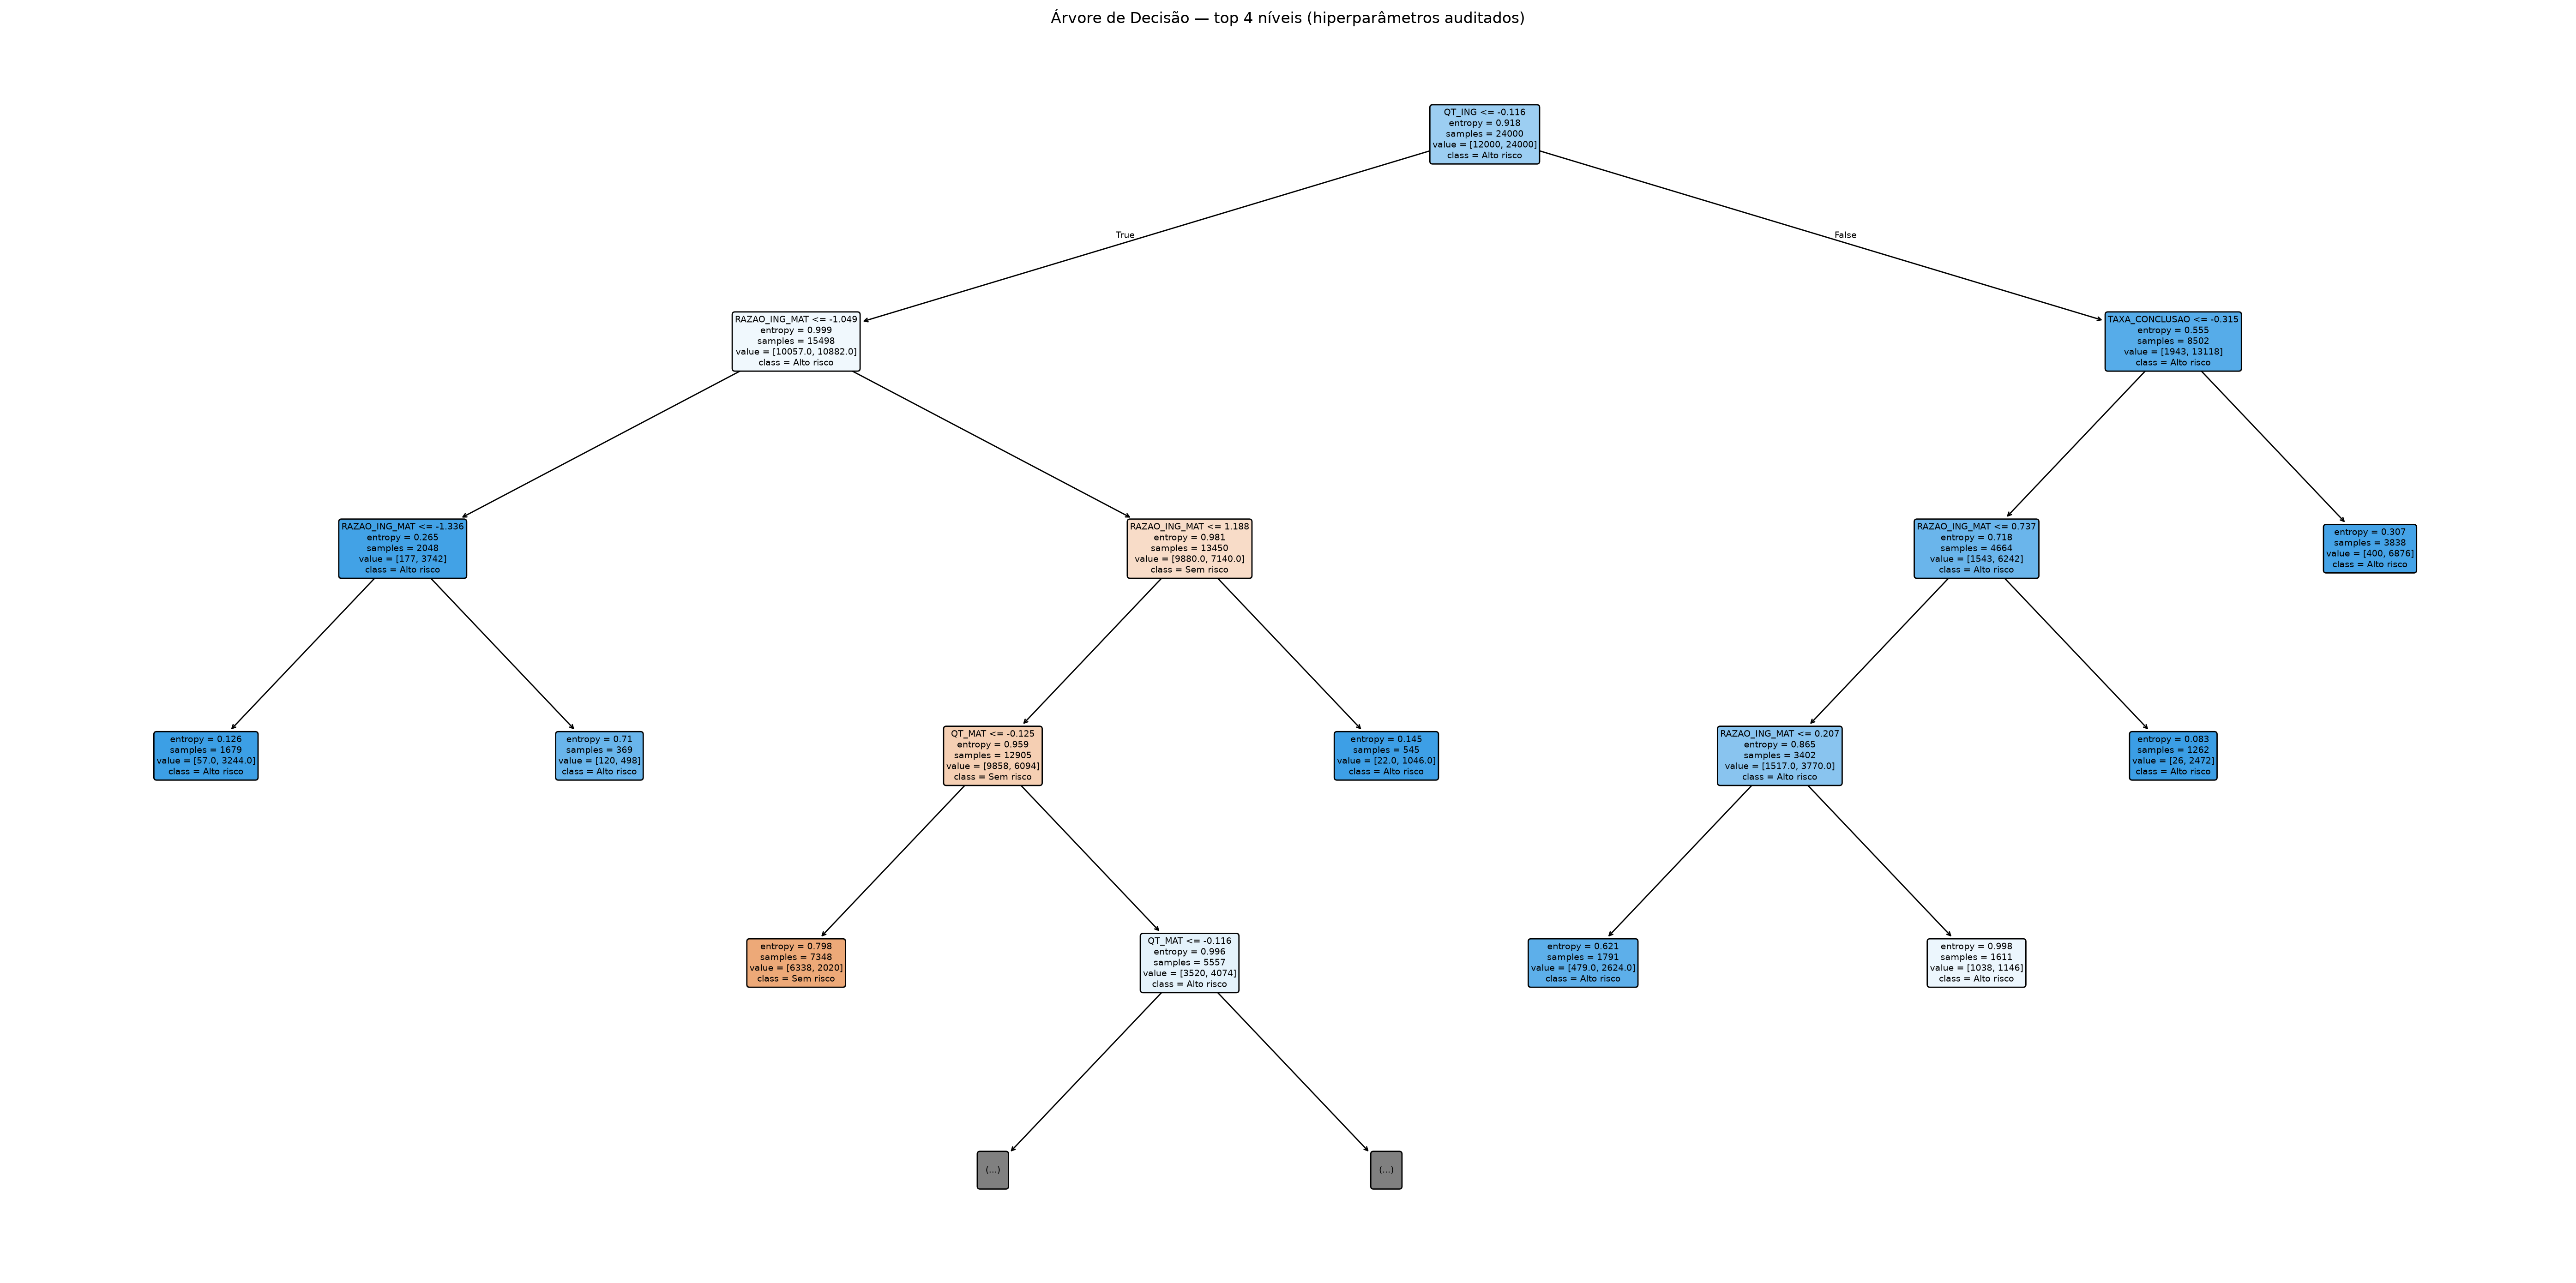
\includegraphics[width=\textwidth]{decision_tree/decision_tree_final.png}
\caption{Visualização da árvore de decisão ajustada sob protocolo auditado. Variáveis em escala padronizada; folhas indicam classe predita (\texttt{class: 0} = baixo risco, \texttt{class: 1} = alto risco).}
\label{fig:tree}
\end{figure}


\end{document}
